% Provenance (never printed): old premiere S material on the formation of fossil
% fuels (preserved organic matter, burial, oil window, migration, trap, coal).
% Burial history of the invented Merrow Basin from figdata/grade-11/oil_window.py
% (constant geotherm, no compaction). Rifts and passive margins after the USGS
% West-Central Coastal Province fact sheet (2023-3028). Folds are defined in
% g12.02 mountain-building (Sync 0): the anticline is told in prose here, never
% defined. Sedimentary basins compared, diagenesis: Year 1/2.
\chapter{A geologia do carvão, do petróleo e do gás}\label{ch:g11:fossil-fuel-geology}

Uma placa de folhelho negro tirada de uma antiga mina de \omterm{def:g11:fossil-fuel-geology:coal}{carvão} na
Pensilvânia traz as folhas de plantas parecidas com samambaias, achatadas e
prateadas contra a rocha escura. Elas cresceram num pântano há mais de
trezentos milhões de anos, no Carbonífero; enterradas antes de apodrecer,
conservaram a sua forma, e o carbono das plantas do pântano virou \omterm{def:g11:fossil-fuel-geology:coal}{carvão}. O
petróleo e o gás, bombeados hoje de plataformas em alto-mar, têm o mesmo
tipo de origem: os restos de seres vivos que escaparam da decomposição e
depois foram enterrados e aquecidos. Este capítulo acompanha esse carbono
enterrado, do pântano e do fundo do mar até a camada de \omterm{def:g11:fossil-fuel-geology:coal}{carvão} e o campo de
petróleo.
% ledger: photo:g11-fossil-plants, ics:base.Carboniferous, ics:base.Permian, earle:coal-formation, earle:organic-preservation

\begin{omfigure}
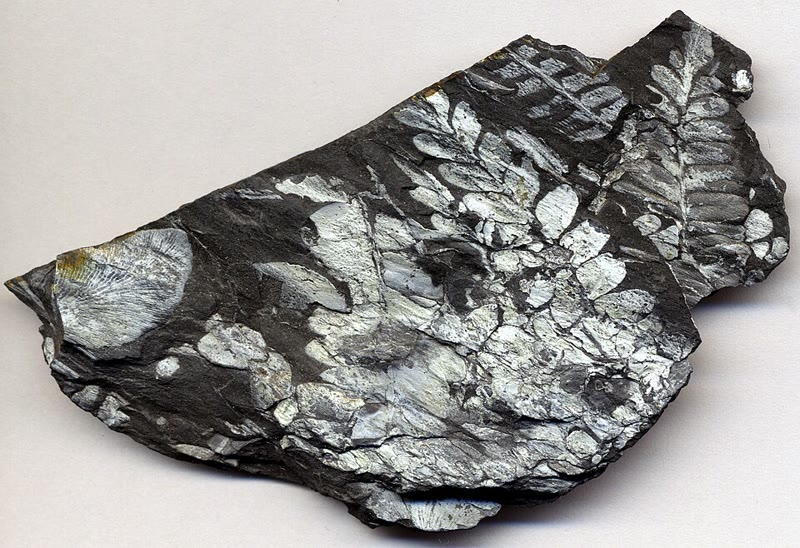
\includegraphics[height=4.4cm]{images/book2/g11-stjohn-fossil-plants.jpg}\hspace{0.03\linewidth}%
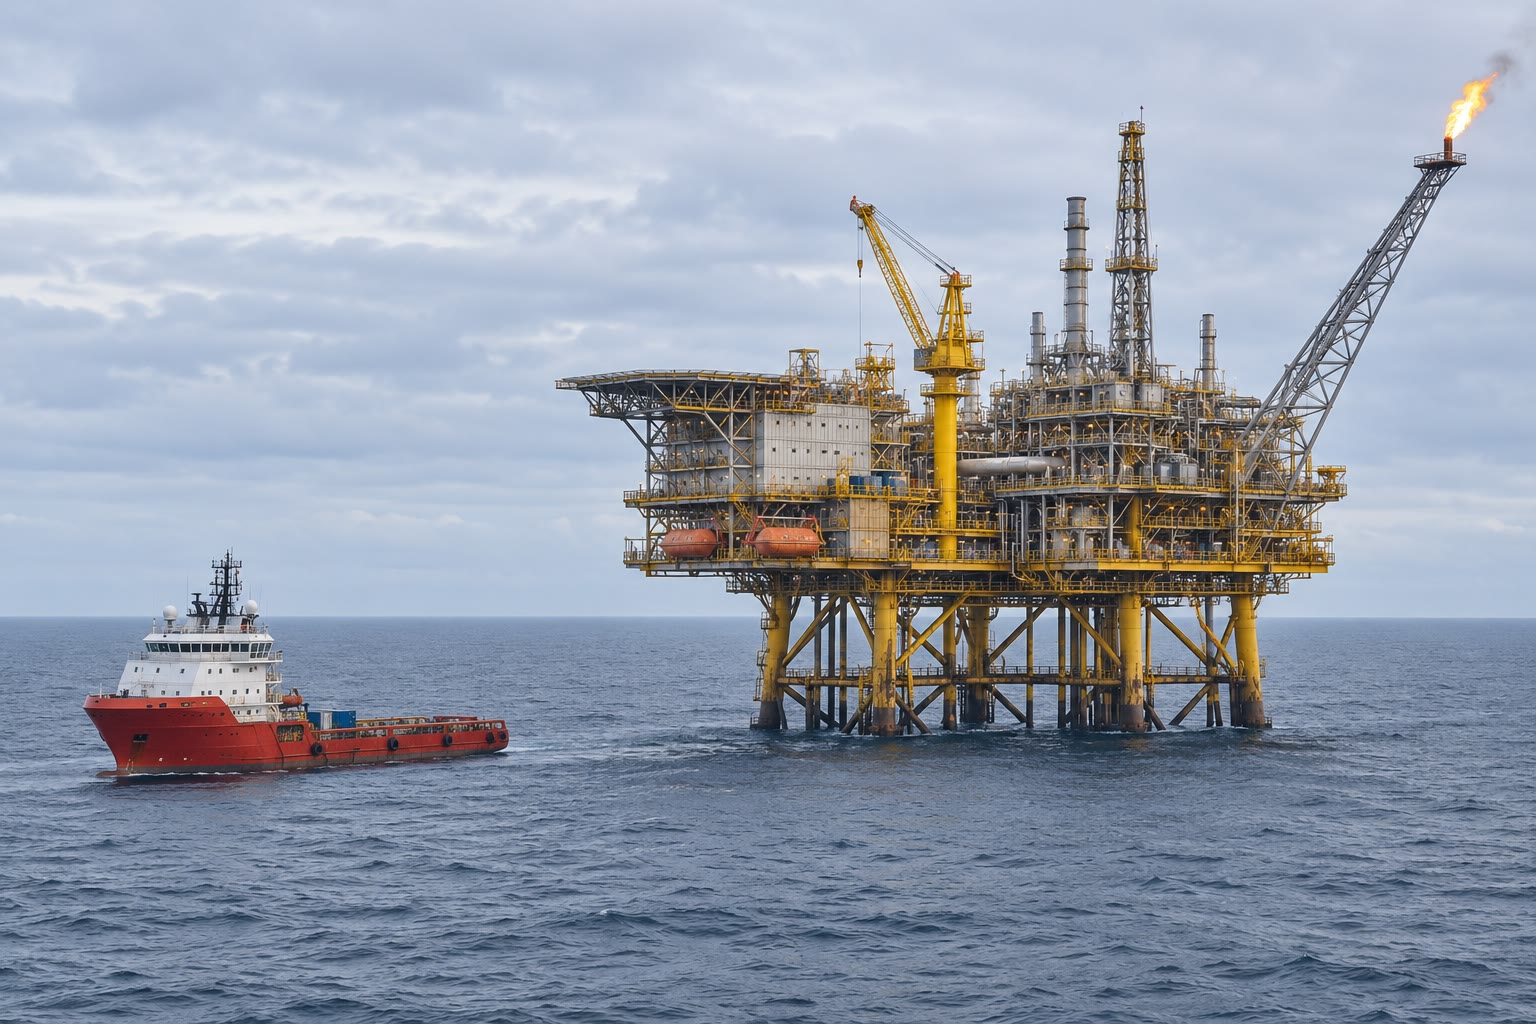
\includegraphics[height=4.4cm]{images/book2/ai/g11-offshore-platform.jpg}

{\small À esquerda: folhas de plantas fósseis num folhelho rico em carbono
de uma antiga mina de \omterm{def:g11:fossil-fuel-geology:coal}{carvão}, na Pensilvânia, do Carbonífero; a placa tem
cerca de \qty{10}{cm} de largura. Fotografia James St.~John (CC~BY~2.0). À
direita: uma plataforma de produção de petróleo e gás no mar (ilustração
gerada por IA).}
\end{omfigure}
% ledger: photo:g11-fossil-plants

\begin{recall}
O \omterm{def:g11:fossil-fuel-geology:coal}{carvão}, o petróleo e o gás natural são combustíveis fósseis: o petróleo e o
gás são misturas de hidrocarbonetos, compostos de carbono e hidrogênio, e
queimar um combustível fóssil libera energia e gás carbônico (os livros de
química). As plantas e as algas produzem matéria orgânica a partir de gás
carbônico e água pela fotossíntese (os livros de biologia). O \omterm{def:g11:fossil-fuel-geology:coal}{carvão}, o
petróleo e o gás vêm de matéria orgânica enterrada em sedimentos, e ficam
armazenados em rochas sedimentares (Livro 1, 9º ano). Uma rocha é porosa
quando contém espaços vazios, e permeável quando a água pode escoar através
dela (Livro 1, 6º ano). A temperatura sobe com a profundidade ao longo da
\omterm{def:g11:lithosphere-asthenosphere:geotherm}{geoterma}, de 25 a \qty{30}{\degreeCelsius} por quilômetro nos primeiros
quilômetros (\cref{ch:g11:lithosphere-asthenosphere}).
\end{recall}
% ledger: usgs:gradient-29, earle:organic-preservation

\section{Conservar a matéria orgânica}

A maior parte da matéria orgânica nunca vira combustível. Uma folha morta ou
uma alga morta é comida por animais e bactérias, ou reage com o oxigênio do
ar: em semanas ou anos, o seu carbono volta à atmosfera como gás carbônico.
A matéria orgânica só sobrevive onde fica isolada do oxigênio --- no fundo de
um pântano de água parada, ou num fundo de mar ou de lago cuja água não
contém oxigênio. Enterrada ali sob mais sedimento, ela pode se conservar por
dezenas ou centenas de milhões de anos.
% ledger: earle:organic-preservation

O \omterm{def:g11:fossil-fuel-geology:coal}{carvão} vem principalmente de plantas terrestres que se acumularam em
pântanos. O petróleo e o gás vêm principalmente das algas microscópicas e de
outros organismos do plâncton do mar: onde as águas de superfície são muito
produtivas, o plâncton morto chove sobre o fundo do mar depressa o bastante
para que uma parte escape da decomposição, e ele é enterrado na lama.
% ledger: earle:coal-formation, earle:oil-window

\begin{definition}[Rocha geradora; querogênio]\label{def:g11:fossil-fuel-geology:source-rock}
O \emph{querogênio}\index{querogenio@querogênio} é a matéria orgânica
dispersa numa rocha sedimentar, em pequenas partículas que não se dissolvem
em solventes orgânicos. Uma \emph{rocha geradora}\index{rocha geradora} é
uma rocha sedimentar rica em querogênio, na qual o petróleo e o gás se
formam quando ela é enterrada e aquecida.
\end{definition}
% ledger: peters08:kerogen, earle:migration-traps

A maioria das \omterm{def:g11:fossil-fuel-geology:source-rock}{rochas geradoras} são folhelhos e lamitos, depositados como
lamas ricas em matéria orgânica. Perto da superfície, o seu \omterm{def:g11:fossil-fuel-geology:source-rock}{querogênio}
continua sólido: bactérias que vivem sem oxigênio transformam parte da
matéria orgânica em metano, mas a maior parte desse metano escapa de volta
para a superfície. Produzir petróleo exige calor, e o calor exige profundidade.
% ledger: earle:oil-window, peters08:kerogen

\section{Soterramento e maturação}

\begin{definition}[Bacia sedimentar]\label{def:g11:fossil-fuel-geology:basin}
Uma \emph{bacia sedimentar}\index{bacia sedimentar} é uma região da crosta
que afunda ao longo de milhões de anos, de modo que os sedimentos se
acumulam nela, muitas vezes com vários quilômetros de espessura.
\end{definition}
% ledger: usgs23:rift-salt

Numa bacia que afunda, cada camada é enterrada cada vez mais fundo sob as
camadas que se acumulam por cima dela. À medida que desce, ela segue a
\omterm{def:g11:lithosphere-asthenosphere:geotherm}{geoterma}: ela é aquecida. O seu \omterm{def:g11:fossil-fuel-geology:source-rock}{querogênio} é lentamente cozido, e as suas
grandes moléculas são quebradas nas moléculas menores do petróleo e do gás.
% ledger: earle:oil-window

\begin{definition}[Maturação; janela do petróleo; janela do gás]\label{def:g11:fossil-fuel-geology:oil-window}
A \emph{maturação}\index{maturacao@maturação} de uma \omterm{def:g11:fossil-fuel-geology:source-rock}{rocha geradora} é a
transformação do seu \omterm{def:g11:fossil-fuel-geology:source-rock}{querogênio} em petróleo e gás à medida que ela é
enterrada e aquecida. A \emph{janela do petróleo}\index{janela do petroleo@janela do petróleo} é a faixa de
temperatura, de cerca de 60 a \qty{120}{\degreeCelsius}, na qual o
\omterm{def:g11:fossil-fuel-geology:source-rock}{querogênio} forma principalmente petróleo. Acima de cerca de
\qty{120}{\degreeCelsius}, na \emph{janela do
gás}\index{janela do gas@janela do gás}, ele forma principalmente metano.
\end{definition}
% ledger: earle:oil-window, magoon00:tps

Como a temperatura sobe com a profundidade, a \omterm{def:g11:fossil-fuel-geology:oil-window}{janela do petróleo} é também
uma faixa de profundidades. Onde a \omterm{def:g11:lithosphere-asthenosphere:geotherm}{geoterma} é uma reta, é fácil encontrá-la.

\begin{proposition}[Profundidade da janela do petróleo]\label{prop:g11:fossil-fuel-geology:window-depth}
Seja $T_0$ a temperatura na superfície, que sobe com a profundidade $z$ com
um \omterm{def:g11:lithosphere-asthenosphere:geotherm}{gradiente geotérmico} constante $G$: $T = T_0 + G z$. Então a \omterm{def:g11:fossil-fuel-geology:oil-window}{janela do
petróleo} fica entre as profundidades
\[
  z_{\text{topo}} = \frac{60 - T_0}{G}
  \qquad\text{e}\qquad
  z_{\text{base}} = \frac{120 - T_0}{G},
\]
com as temperaturas em \unit{\degreeCelsius}. A sua espessura é $60/G$:
quanto mais íngreme a \omterm{def:g11:lithosphere-asthenosphere:geotherm}{geoterma}, mais rasa e mais fina a janela.
\end{proposition}
% ledger: earle:oil-window

\begin{proof}
O topo da janela é a profundidade em que $T_0 + G z = 60$, isto é,
$z = (60 - T_0)/G$; a base fica onde $T_0 + G z = 120$. A diferença é
$(120 - 60)/G = 60/G$.
\end{proof}

Com uma superfície a \qty{20}{\degreeCelsius} e um gradiente de
\qty{30}{\degreeCelsius} por quilômetro, a \omterm{def:g11:fossil-fuel-geology:oil-window}{janela do petróleo} fica entre
$40/30 \approx \qty{1.3}{km}$ e $100/30 \approx \qty{3.3}{km}$. Nos furos
de sondagem dos Estados Unidos, o gradiente é em média de
\qty{29}{\degreeCelsius} por quilômetro, \num{25} no leste e \num{34} no
oeste; uma \omterm{def:g11:fossil-fuel-geology:source-rock}{rocha geradora} em geral precisa ser enterrada a mais de cerca de
\qty{2}{km} antes de produzir petróleo. Quando não há nenhuma medição do
\omterm{def:g11:fossil-fuel-geology:source-rock}{querogênio}, os geólogos do petróleo têm considerado madura uma \omterm{def:g11:fossil-fuel-geology:source-rock}{rocha
geradora} enterrada sob mais de cerca de \qty{3}{km} de rochas mais jovens.
% values (oil_window.py): z_top_km 1.3333, z_base_km 3.3333
% ledger: usgs:gradient-29, earle:oil-window, magoon00:tps

\begin{omfigure}
\begin{tikzpicture}
\begin{axis}[omrecord, omage, omdepth, name=burial, width=0.54\linewidth, height=5.6cm,
  xmin=0, xmax=170, ymin=0, ymax=4.5, xlabel={idade (milhões de anos atrás)},
  ylabel={profundidade (\unit{km})}, unbounded coords=jump, clip=false,
  xtick={0,20,...,160}, ytick={0,1,...,4}]
\fill[omProp!18] (axis cs:170,1.3333) rectangle (axis cs:0,3.3333);
\fill[omThm!12] (axis cs:170,3.3333) rectangle (axis cs:0,4.5);
\node[font=\scriptsize, anchor=west, text=omProp!80!black] at (axis cs:168,1.75) {janela do petróleo};
\node[font=\scriptsize, anchor=west, text=omThm] at (axis cs:168,3.9) {janela do gás};
\node[font=\scriptsize, anchor=south west, text=black!60, inner sep=1pt] at (axis cs:168,1.3333) {\qty{60}{\degreeCelsius}};
\node[font=\scriptsize, anchor=south west, text=black!60, inner sep=1pt] at (axis cs:168,3.3333) {\qty{120}{\degreeCelsius}};
% computed in figdata/grade-11/oil_window.py (invented basin)
\addplot[black!45, line width=0.6pt] table[x=age, y=z150] {figdata/out/grade-11-oil_window-history.dat};
\addplot[black!45, line width=0.6pt] table[x=age, y=z120] {figdata/out/grade-11-oil_window-history.dat};
\addplot[black!45, line width=0.6pt] table[x=age, y=z95] {figdata/out/grade-11-oil_window-history.dat};
\addplot[black!45, line width=0.6pt] table[x=age, y=z66] {figdata/out/grade-11-oil_window-history.dat};
\addplot[black, line width=1.4pt] table[x=age, y=z165] {figdata/out/grade-11-oil_window-history.dat};
\draw[omDef, dashed, line width=0.8pt] (axis cs:80,0) -- (axis cs:80,4.5);
\node[font=\scriptsize, anchor=west, text=omDef, inner sep=1pt] at (axis cs:78,4.2) {forma-se o anticlinal};
\fill[omThm] (axis cs:116.97,1.3333) circle (2pt);
\fill[omThm] (axis cs:51.24,3.3333) circle (2pt);
\node[font=\scriptsize, anchor=north east, inner sep=1pt] at (axis cs:100,2.3) {rocha geradora};
\end{axis}
\begin{axis}[omrecord, omdepth, at={(burial.east)}, anchor=west, xshift=1.7cm, width=0.34\linewidth, height=5.6cm,
  xmin=15, xmax=50, ymin=0, ymax=7, xlabel={gradiente (\unit{\degreeCelsius/km})},
  ylabel={profundidade (\unit{km})}]
% computed in figdata/grade-11/oil_window.py (proposition, surface at 20 degC)
\addplot[name path=top, omProp, line width=1pt] table[x=G, y=z_top] {figdata/out/grade-11-oil_window-windows.dat};
\addplot[name path=base, omThm, line width=1pt] table[x=G, y=z_base] {figdata/out/grade-11-oil_window-windows.dat};
\addplot[omProp!18] fill between[of=top and base];
\node[font=\scriptsize] at (axis cs:40,1.75) {janela do petróleo};
\node[font=\scriptsize, anchor=south, text=omProp!80!black] at (axis cs:42,0.95) {topo};
\node[font=\scriptsize, anchor=north west, text=omThm] at (axis cs:24,4.6) {base};
\end{axis}
\end{tikzpicture}

{\small À esquerda: história de soterramento da Bacia de Merrow, uma bacia
inventada (modelo calculado, sem levar em conta a compactação). Cada linha
segue uma camada ao longo do tempo, a partir do dia em que ela foi
depositada na superfície; a linha grossa é a \omterm{def:g11:fossil-fuel-geology:source-rock}{rocha geradora}, depositada há
165 milhões de anos. Com a superfície a \qty{20}{\degreeCelsius} e um
gradiente de \qty{30}{\degreeCelsius} por quilômetro, a \omterm{def:g11:fossil-fuel-geology:oil-window}{janela do petróleo} é
a faixa entre \num{1.3} e \qty{3.3}{km}. Os pontos marcam quando a \omterm{def:g11:fossil-fuel-geology:source-rock}{rocha
geradora} entrou nela e quando saiu dela para a \omterm{def:g11:fossil-fuel-geology:oil-window}{janela do gás}. À direita:
profundidade do topo e da base da \omterm{def:g11:fossil-fuel-geology:oil-window}{janela do petróleo} em função do \omterm{def:g11:lithosphere-asthenosphere:geotherm}{gradiente
geotérmico} (superfície a \qty{20}{\degreeCelsius}).}
\end{omfigure}
% values (oil_window.py): enter_oil_Ma 116.97, leave_oil_Ma 51.24, T_max 140 (20 Ma), T_today 125

Um diagrama como este é um \emph{diagrama de história de soterramento}: a
idade avança da esquerda para a direita em direção a hoje, a profundidade
para baixo. Ele transforma uma coluna de rochas, datada camada por camada,
numa história.

\begin{method}[Ler um diagrama de história de soterramento]\label{met:g11:fossil-fuel-geology:burial}
\begin{enumerate}
  \item Encontre a linha da \omterm{def:g11:fossil-fuel-geology:source-rock}{rocha geradora}: ela começa na superfície no dia
        em que a rocha foi depositada.
  \item Trace o topo e a base da \omterm{def:g11:fossil-fuel-geology:oil-window}{janela do petróleo}, como profundidades, a
        partir da \omterm{def:g11:lithosphere-asthenosphere:geotherm}{geoterma} (\cref{prop:g11:fossil-fuel-geology:window-depth}).
  \item Leia a idade em que a linha da \omterm{def:g11:fossil-fuel-geology:source-rock}{rocha geradora} cruza o topo da
        janela: a \omterm{def:g11:fossil-fuel-geology:source-rock}{rocha geradora} começa a produzir petróleo. Leia a idade em
        que ela cruza a base: a partir daí, ela produz gás.
  \item Compare essas idades com a idade da \omterm{def:g11:fossil-fuel-geology:trap}{armadilha}: só o petróleo e o gás
        formados depois que a \omterm{def:g11:fossil-fuel-geology:trap}{armadilha} existe podem ficar retidos nela.
\end{enumerate}
\end{method}
% ledger: magoon00:tps

Na Bacia de Merrow, a \omterm{def:g11:fossil-fuel-geology:source-rock}{rocha geradora} entra na \omterm{def:g11:fossil-fuel-geology:oil-window}{janela do petróleo} há cerca de
117 milhões de anos e sai dela há cerca de 51 milhões de anos; o seu
soterramento máximo, \qty{4.0}{km} a \qty{140}{\degreeCelsius}, acontece há
20 milhões de anos, antes que o soerguimento e a erosão a façam subir de
novo. Hoje ela ainda está na \omterm{def:g11:fossil-fuel-geology:oil-window}{janela do gás}. O problema de fim de semana
calcula essas idades.
% values (oil_window.py): enter_oil_Ma 116.97, leave_oil_Ma 51.24, z_max_km 4, T_max 140, T_today 125

\section{Da rocha geradora à armadilha}

O petróleo e o gás são mais leves que a água, e os poros das rochas
enterradas estão cheios de água. Uma vez formados, eles são expulsos da
\omterm{def:g11:fossil-fuel-geology:source-rock}{rocha geradora} e sobem lentamente, através de qualquer rocha que os deixe
passar.
% ledger: earle:migration-traps

\begin{definition}[Migração]\label{def:g11:fossil-fuel-geology:migration}
A \emph{migração}\index{migracao (do petroleo e do gas)@migração (do petróleo e do gás)} é o movimento lento do
petróleo e do gás para fora da \omterm{def:g11:fossil-fuel-geology:source-rock}{rocha geradora} onde se formaram, para cima
através de rochas permeáveis, impulsionado pela sua densidade menor que a da
água em volta.
\end{definition}
% ledger: earle:migration-traps

\begin{definition}[Rocha reservatório; rocha selante]\label{def:g11:fossil-fuel-geology:reservoir}
Uma \emph{rocha reservatório}\index{rocha reservatorio@rocha reservatório} é
uma rocha porosa e permeável na qual o petróleo e o gás se acumulam: os seus
poros os armazenam, e as ligações entre os poros os deixam escoar até um
poço. Uma \emph{rocha selante}\index{rocha selante} é uma rocha impermeável
acima do reservatório, através da qual o petróleo e o gás não podem passar.
\end{definition}
% ledger: earle:migration-traps, magoon00:tps

Os arenitos e alguns calcários são bons reservatórios; os lamitos, os
folhelhos e o sal são boas \omterm{def:g11:fossil-fuel-geology:reservoir}{rochas selantes}. Onde nada os detém, o petróleo e
o gás chegam à superfície, onde exsudam e são oxidados: o seu carbono volta
à atmosfera. Eles só se acumulam onde uma \omterm{def:g11:fossil-fuel-geology:reservoir}{rocha selante} tem uma forma que
não os deixa escapar por baixo dela.
% ledger: earle:migration-traps, magoon00:tps

\begin{definition}[Armadilha]\label{def:g11:fossil-fuel-geology:trap}
Uma \emph{armadilha}\index{armadilha (petroleo e gas)@armadilha (petróleo e gás)} é um arranjo de \omterm{def:g11:fossil-fuel-geology:reservoir}{rocha
reservatório} e de \omterm{def:g11:fossil-fuel-geology:reservoir}{rocha selante} que retém o petróleo e o gás no lugar,
fechando o caminho para cima por todos os lados.
\end{definition}
% ledger: earle:migration-traps

\begin{omfigure}
\begin{tikzpicture}[font=\footnotesize, scale=0.95,
    declare function={hz(\x,\c)=\c+0.1*\x+0.7*exp(-((\x-10)^2)/2.5);}]
  \colorlet{omOil}{green!45!black}\colorlet{omGas}{red!65}
  \fill[omLithShale!70!white] (0,0) rectangle (14,-6.3);
  % overburden: limestone above a sandstone
  \fill[omLithCongl!70!white] (0,0) -- (14,0) -- plot[domain=14:0, samples=80] (\x,{-2.4+0.06*\x+0.3*exp(-((\x-10)^2)/2.5)}) -- cycle;
  \fill[omLithSand!60!white] plot[domain=0:14, samples=80] (\x,{-2.4+0.06*\x+0.3*exp(-((\x-10)^2)/2.5)}) -- plot[domain=14:0, samples=80] (\x,{hz(\x,-3.7)}) -- cycle;
  % seal (mudstone)
  \fill[omLithShale] plot[domain=0:14, samples=80] (\x,{hz(\x,-3.7)}) -- plot[domain=14:0, samples=80] (\x,{hz(\x,-4.4)}) -- cycle;
  % reservoir sandstone
  \fill[omLithSand] plot[domain=0:14, samples=80] (\x,{hz(\x,-4.4)}) -- plot[domain=14:0, samples=80] (\x,{hz(\x,-5.0)}) -- cycle;
  % oil and gas in the crest of the anticline, above the spill depth
  \begin{scope}
    \clip plot[domain=0:14, samples=80] (\x,{hz(\x,-4.4)}) -- plot[domain=14:0, samples=80] (\x,{hz(\x,-5.0)}) -- cycle;
    \fill[omOil] (8,-2.97) rectangle (13,-2.6);
    \fill[omGas] (8,-2.81) rectangle (13,-2.6);
  \end{scope}
  % source rock (black shale)
  \fill[black!70] plot[domain=0:14, samples=80] (\x,{hz(\x,-5.0)}) -- plot[domain=14:0, samples=80] (\x,{hz(\x,-5.6)}) -- cycle;
  \foreach \c in {-3.7,-4.4,-5.0,-5.6}
    \draw[black!55, line width=0.4pt] plot[domain=0:14, samples=80] (\x,{hz(\x,\c)});
  \draw[black!55, line width=0.4pt] plot[domain=0:14, samples=80] (\x,{-2.4+0.06*\x+0.3*exp(-((\x-10)^2)/2.5)});
  \draw[black!70] (0,0) -- (14,0);
  % 60 degC isotherm
  \draw[omThm, dashed, line width=0.8pt] (0,-4.3) -- (14,-4.3);
  \node[anchor=north east, text=omThm, fill=omLithShale!70!white, inner sep=1pt] at (13.95,-4.35) {\qty{60}{\degreeCelsius}};
  % migration
  \foreach \s in {0,1}
    \draw[->, omDef, line width=1.1pt] (2.7+1.2*\s,{-5.1+0.12*\s}) -- (3.2+1.2*\s,{-4.55+0.12*\s});
  \draw[->, omDef, line width=1.1pt] (4.6,-4.3) .. controls (6.5,-4.1) and (8.3,-3.7) .. (9.45,-3.0);
  % labels
  \node[anchor=west, text=white] at (0.15,-5.25) {rocha geradora};
  \node[anchor=west] at (5.2,-5.75) {madura onde é mais quente que \qty{60}{\degreeCelsius}};
  \node[anchor=west] at (0.15,-4.75) {reservatório};
  \node[anchor=west] at (0.15,-3.97) {rocha selante};
  \node[anchor=west] at (0.15,-0.4) {sobrecarga};
  \node[anchor=north, text=omDef, fill=omLithShale, inner sep=1pt] at (6.2,-3.62) {migração};
  \draw[black!60] (10.0,-2.72) -- (11.4,-1.95);
  \node[anchor=south west, fill=omLithSand!60!white, inner sep=1pt] at (11.4,-1.95) {gás};
  \draw[black!60] (10.6,-2.88) -- (12.3,-2.55);
  \node[anchor=west, fill=omLithShale, inner sep=1pt] at (12.3,-2.55) {petróleo};
  \draw[black!60] (12.0,-3.45) -- (12.8,-3.15);
  \node[anchor=south, fill=omLithShale, inner sep=1pt] at (12.85,-3.15) {água};
  \node[anchor=north] at (10,-1.0) {armadilha: o arco de um anticlinal};
\end{tikzpicture}

{\small Um \omterm{def:g11:fossil-fuel-geology:petroleum-system}{sistema petrolífero} (um desenho, fora de escala). A \omterm{def:g11:fossil-fuel-geology:source-rock}{rocha
geradora}, no fundo, à esquerda, fica abaixo da isoterma de
\qty{60}{\degreeCelsius} e produz petróleo; o petróleo e o gás saem dela
para o arenito de cima e sobem lentamente ao longo dele, sob a \omterm{def:g11:fossil-fuel-geology:reservoir}{rocha selante}
de lamito, até o arco de um anticlinal. Ali eles se separam pela densidade:
o gás em cima, o petróleo embaixo, a água mais abaixo. As \omterm{def:g11:fossil-fuel-geology:petroleum-system}{rochas de
sobrecarga}, por cima, enterram a \omterm{def:g11:fossil-fuel-geology:source-rock}{rocha geradora} a uma profundidade
suficiente para que ela amadureça.}
\end{omfigure}
% ledger: earle:migration-traps, magoon00:tps, earle:oil-window

Numa \omterm{def:g11:fossil-fuel-geology:trap}{armadilha}, os fluidos se separam pela densidade: o gás em cima, o
petróleo embaixo, a água no fundo. A \omterm{def:g11:fossil-fuel-geology:trap}{armadilha} mais simples é um anticlinal,
um arco nas camadas (as dobras são assunto do
\cref{ch:g12:mountain-building}). Falhas, domos de sal e mudanças nas
próprias rochas também formam \omterm{def:g11:fossil-fuel-geology:trap}{armadilhas}.
% ledger: earle:migration-traps

\begin{omfigure}
\begin{tikzpicture}[font=\footnotesize, scale=0.78]
  \colorlet{omOil}{green!45!black}\colorlet{omGas}{red!65}
  % (a) anticline
  \begin{scope}
    \fill[omLithShale] (0,0) rectangle (4,3);
    \fill[omLithSand] plot[domain=0:4, samples=50] (\x,{1.0+1.0*exp(-((\x-2)^2)/1.2)}) -- plot[domain=4:0, samples=50] (\x,{1.5+1.0*exp(-((\x-2)^2)/1.2)}) -- cycle;
    \begin{scope}
      \clip plot[domain=0:4, samples=50] (\x,{1.0+1.0*exp(-((\x-2)^2)/1.2)}) -- plot[domain=4:0, samples=50] (\x,{1.5+1.0*exp(-((\x-2)^2)/1.2)}) -- cycle;
      \fill[omOil] (0,1.75) rectangle (4,3); \fill[omGas] (0,2.25) rectangle (4,3);
    \end{scope}
    \draw[black!50] (0,0) rectangle (4,3);
    \node[anchor=north, text height=1.6ex, text depth=0.3ex] at (2,-0.05) {(a) anticlinal};
  \end{scope}
  % (b) fault
  \begin{scope}[xshift=4.6cm]
    \fill[omLithShale] (0,0) rectangle (4,3);
    \begin{scope}
      \clip (0,0) -- (2.9,0) -- (2.3,3) -- (0,3) -- cycle;
      \fill[omLithSand] (0,0.6) -- (4,1.8) -- (4,2.3) -- (0,1.1) -- cycle;
      \clip (0,0.6) -- (4,1.8) -- (4,2.3) -- (0,1.1) -- cycle;
      \fill[omOil] (0,1.45) rectangle (4,3); \fill[omGas] (0,1.75) rectangle (4,3);
    \end{scope}
    \begin{scope}
      \clip (2.9,0) -- (4,0) -- (4,3) -- (2.3,3) -- cycle;
      \fill[omLithSand] (0,-0.6) -- (4,0.6) -- (4,1.1) -- (0,-0.1) -- cycle;
    \end{scope}
    \draw[black, line width=1pt] (2.9,0) -- (2.3,3);
    \draw[black!50] (0,0) rectangle (4,3);
    \node[anchor=north, text height=1.6ex, text depth=0.3ex] at (2,-0.05) {(b) falha};
  \end{scope}
  % (c) salt dome
  \begin{scope}[xshift=9.2cm]
    \fill[omLithShale] (0,0) rectangle (4,3);
    \fill[omLithSand] (0,0.9) -- (1.0,1.2) -- (1.4,1.9) -- (1.4,2.4) -- (1.0,1.7) -- (0,1.4) -- cycle;
    \fill[omLithSand] (4,0.9) -- (3.0,1.2) -- (2.6,1.9) -- (2.6,2.4) -- (3.0,1.7) -- (4,1.4) -- cycle;
    \begin{scope}
      \clip (0,0.9) -- (1.0,1.2) -- (1.4,1.9) -- (1.4,2.4) -- (1.0,1.7) -- (0,1.4) -- cycle;
      \fill[omOil] (0,1.65) rectangle (1.4,3); \fill[omGas] (0,2.05) rectangle (1.4,3);
    \end{scope}
    \begin{scope}
      \clip (4,0.9) -- (3.0,1.2) -- (2.6,1.9) -- (2.6,2.4) -- (3.0,1.7) -- (4,1.4) -- cycle;
      \fill[omOil] (2.6,1.65) rectangle (4,3); \fill[omGas] (2.6,2.05) rectangle (4,3);
    \end{scope}
    \fill[omLithEvap, draw=black!60] (1.4,0) -- (1.4,2.4) .. controls (1.4,2.85) and (2.6,2.85) .. (2.6,2.4) -- (2.6,0) -- cycle;
    \node at (2,1.0) {sal};
    \draw[black!50] (0,0) rectangle (4,3);
    \node[anchor=north, text height=1.6ex, text depth=0.3ex] at (2,-0.05) {(c) domo de sal};
  \end{scope}
  % (d) stratigraphic
  \begin{scope}[xshift=13.8cm]
    \fill[omLithShale] (0,0) rectangle (4,3);
    \fill[omLithSand] (0,0.6) -- (3.5,1.95) -- (0,1.3) -- cycle;
    \begin{scope}
      \clip (0,0.6) -- (3.5,1.95) -- (0,1.3) -- cycle;
      \fill[omOil] (0,1.45) rectangle (4,3); \fill[omGas] (0,1.7) rectangle (4,3);
    \end{scope}
    \draw[black!50] (0,0) rectangle (4,3);
    \node[anchor=north, text height=1.6ex, text depth=0.3ex] at (2,-0.05) {(d) acunhamento};
  \end{scope}
\end{tikzpicture}

{\small Quatro tipos de \omterm{def:g11:fossil-fuel-geology:trap}{armadilha} (desenhos, fora de escala): o arenito
reservatório em amarelo, o lamito selante em cinza-esverdeado, o petróleo em
verde, o gás em vermelho. (a) O arco de um anticlinal. (b) Um reservatório
inclinado cortado por uma falha, contra um lamito do outro lado. (c) Camadas
dobradas para cima contra um domo de sal que sobe. (d) Um arenito que se
afina encosta acima dentro de um lamito, uma \omterm{def:g11:fossil-fuel-geology:trap}{armadilha} produzida por uma
mudança nas próprias rochas.}
\end{omfigure}
% ledger: earle:migration-traps

\begin{example}[Uma armadilha num anticlinal]\label{ex:g11:fossil-fuel-geology:anticline}
Um levantamento sísmico mapeia o topo de um arenito selado por lamito. Ele
forma um arco cuja crista fica a \qty{1800}{m} abaixo da superfície. Em
volta da crista, a curva de nível mais profunda que ainda se fecha
completamente fica a \qty{2050}{m}; abaixo dela, o arenito se abre para o
lado. Um poço na crista encontra gás até \qty{1880}{m}. Que altura de
coluna de petróleo e gás a \omterm{def:g11:fossil-fuel-geology:trap}{armadilha} pode conter, e qual é a espessura do
petróleo?

\emph{Solução.} O petróleo e o gás enchem o arco da crista para baixo; o que
desce abaixo da última curva de nível fechada transborda para o lado, no
\emph{ponto de derrame}, e continua a migrar. A coluna tem no máximo
$2050 - 1800 = \qty{250}{m}$ de altura. Se a \omterm{def:g11:fossil-fuel-geology:trap}{armadilha} está cheia, o gás
ocupa os $1880 - 1800 = \qty{80}{m}$ de cima e o petróleo os
$2050 - 1880 = \qty{170}{m}$ seguintes, com água abaixo.
\end{example}
% invented numbers; ledger: earle:migration-traps

Cada uma das peças --- uma \omterm{def:g11:fossil-fuel-geology:source-rock}{rocha geradora}, um reservatório, uma \omterm{def:g11:fossil-fuel-geology:reservoir}{rocha
selante}, as rochas de cima que enterram a \omterm{def:g11:fossil-fuel-geology:source-rock}{rocha geradora}, uma \omterm{def:g11:fossil-fuel-geology:trap}{armadilha} ---
é necessária, e elas precisam vir na ordem certa.

\begin{definition}[Sistema petrolífero]\label{def:g11:fossil-fuel-geology:petroleum-system}
Um \emph{sistema petrolífero}\index{sistema petrolifero@sistema petrolífero}
é um corpo de \omterm{def:g11:fossil-fuel-geology:source-rock}{rocha geradora} madura com todo o petróleo e o gás que saíram
dele, e os elementos e processos de que eles precisam: a \omterm{def:g11:fossil-fuel-geology:source-rock}{rocha geradora}, a
\omterm{def:g11:fossil-fuel-geology:reservoir}{rocha reservatório}, a \omterm{def:g11:fossil-fuel-geology:reservoir}{rocha selante} e as \emph{rochas de
sobrecarga}\index{rochas de sobrecarga} (as rochas de cima, que enterram a
\omterm{def:g11:fossil-fuel-geology:source-rock}{rocha geradora}), e a formação das \omterm{def:g11:fossil-fuel-geology:trap}{armadilhas}, a geração, a \omterm{def:g11:fossil-fuel-geology:migration}{migração} e a
acumulação do petróleo e do gás.
\end{definition}
% ledger: magoon00:tps

A ordem é o que mais importa. Uma \omterm{def:g11:fossil-fuel-geology:trap}{armadilha} que se forma depois que o
petróleo já passou não captura nada: o diagrama de história de soterramento
data a geração do petróleo, a história das dobras e das falhas data a
\omterm{def:g11:fossil-fuel-geology:trap}{armadilha}, e o \omterm{def:g11:fossil-fuel-geology:petroleum-system}{sistema petrolífero} só funciona se a \omterm{def:g11:fossil-fuel-geology:trap}{armadilha} veio primeiro.
Os geólogos do petróleo também chamam de \emph{momento crítico} o tempo que
melhor mostra a geração, a \omterm{def:g11:fossil-fuel-geology:migration}{migração} e a acumulação juntas.
% ledger: magoon00:tps

\section{Onde o petróleo e o gás se acumulam}

Onde um \omterm{def:g11:fossil-fuel-geology:petroleum-system}{sistema petrolífero} se monta? Ele precisa de uma bacia que afunde
por muito tempo, de águas pobres em oxigênio para conservar a matéria
orgânica, e de \omterm{def:g11:fossil-fuel-geology:reservoir}{rochas selantes}. Os riftes e as margens continentais em que
eles se transformam têm os três.
% ledger: usgs23:rift-salt

Quando um continente começa a se partir, como a África hoje ao longo do
Rifte da África Oriental (Livro 1, 7º ano), a sua crosta se estira e se
quebra em blocos ao longo de \omterm{def:g11:ocean-ridges:normal-fault}{falhas normais} (\cref{ch:g11:ocean-ridges}).
Alguns blocos descem, outros se inclinam, e as depressões entre eles se
enchem de sedimentos, muitas vezes com vários quilômetros de espessura, e de
lagos, cujas lamas ricas em matéria orgânica podem se tornar \omterm{def:g11:fossil-fuel-geology:source-rock}{rochas
geradoras}. Quando
o estiramento para, a crosta afinada esfria e continua a afundar devagar, de
modo que a bacia continua a se encher. Se então o mar invade uma bacia
ligada só em parte ao oceano e evapora, ele deixa espessas camadas de sal.
Depois que o rifte se abriu num oceano, as suas bordas se tornam margens
passivas: bordas de continentes dentro de uma placa, longe de qualquer
limite de placas, que continuam a afundar e a receber sedimentos vindos do
continente.
% ledger: usgs23:rift-salt, usgs:pangaea-breakup

\begin{omfigure}
\begin{tikzpicture}[font=\footnotesize, x=1cm, y=0.8cm]
  \fill[omLithShale] (0,0.25) -- (1.5,0) -- (7,-0.4) -- (10,-2.2) -- (14,-2.6) -- (14,-8.0) -- (0,-8.0) -- cycle;
  % sea and land
  \fill[omSea] (1.5,0) -- (14,0) -- (14,-2.6) -- (10,-2.2) -- (7,-0.4) -- cycle;
  \draw[omRiver!60, line width=0.6pt] (1.5,0) -- (14,0);
  % marine sediments above the salt
  \fill[omLithShale] (0,0.25) -- (1.5,0) -- (7,-0.4) -- (10,-2.2) -- (14,-2.6) -- (14,-4.95) -- (11.2,-4.5) -- (11.2,-3.74) -- (0,-2.4) -- cycle;
  \fill[omLithSand] (0,-0.9) -- (6,-1.45) -- (10,-2.75) -- (14,-3.3) -- (14,-3.6) -- (10,-3.05) -- (6,-1.75) -- (0,-1.2) -- cycle;
  % salt layer and a salt dome
  \fill[omLithEvap, draw=black!50] (1.2,-2.25) -- (11.2,-3.74) -- (11.2,-4.14) -- (1.2,-2.65) -- cycle;
  \fill[omLithEvap, draw=black!50] (7.0,-3.0) .. controls (7.3,-2.6) and (7.25,-1.9) .. (7.2,-1.6)
     .. controls (7.4,-1.2) and (8.2,-1.2) .. (8.4,-1.6)
     .. controls (8.35,-2.1) and (8.3,-2.7) .. (8.7,-3.25) -- cycle;
  % continental crust with tilted blocks
  \fill[omLithGranite] (0,-2.75) -- (2.5,-3.0) -- (4.85,-4.6) -- (5.0,-3.4) -- (7.35,-5.0) -- (7.5,-3.75) -- (9.85,-5.3) -- (10.0,-4.1) -- (11.2,-5.0) -- (11.2,-6.0) -- (0,-7.6) -- cycle;
  % rift fill: lake shales (source rocks) in the half-grabens
  \fill[black!65] (2.5,-3.0) -- (4.85,-4.6) -- (5.0,-3.4) -- (4.0,-3.25) -- cycle;
  \fill[black!65] (5.0,-3.4) -- (7.35,-5.0) -- (7.5,-3.75) -- (6.5,-3.6) -- cycle;
  \fill[black!65] (7.5,-3.75) -- (9.85,-5.3) -- (10.0,-4.1) -- (9.0,-3.95) -- cycle;
  \fill[black!65] (2.5,-3.0) -- (4.0,-3.25) -- (5.0,-3.4) -- (6.5,-3.6) -- (7.5,-3.75) -- (9.0,-3.95) -- (10.0,-4.1) -- (11.2,-4.3) -- (11.2,-4.14) -- (1.2,-2.65) -- (1.2,-2.87) -- cycle;
  \draw[black!70, line width=0.8pt] (4.85,-4.6) -- (5.0,-3.4) (7.35,-5.0) -- (7.5,-3.75) (9.85,-5.3) -- (10.0,-4.1);
  % oceanic crust and mantle
  \fill[omLithBasalt] (11.2,-4.5) -- (14,-4.95) -- (14,-6.0) -- (11.2,-6.0) -- cycle;
  \fill[omLithPeridotite] (0,-7.6) -- (11.2,-6.0) -- (14,-6.0) -- (14,-8.0) -- (0,-8.0) -- cycle;
  % oil beside the salt dome
  \fill[green!45!black] (6.85,-1.5) -- (7.22,-1.65) -- (7.22,-1.95) -- (6.85,-1.75) -- cycle;
  \draw[black!60] (0,-8.0) rectangle (14,1.0);
  % labels
  \node[anchor=west] at (11.5,-1.2) {mar};
  \node[anchor=south west] at (0.1,0.3) {continente};
  \node[anchor=west, fill=omLithShale, inner sep=1pt] at (2.2,-0.45) {sedimentos marinhos};
  \node[anchor=west, fill=omLithEvap, inner sep=1pt] at (9.0,-1.25) {domo de sal};
  \draw[black!60] (8.4,-1.4) -- (9.0,-1.25);
  \node[anchor=east, fill=omLithShale, inner sep=1pt] at (6.6,-2.1) {petróleo};
  \draw[black!60] (6.6,-2.1) -- (6.95,-1.75);
  \node[anchor=west, fill=omLithShale, inner sep=1pt] at (11.4,-3.35) {sal (selante)};
  \draw[black!60] (10.8,-3.7) -- (11.4,-3.35);
  \node[anchor=west, align=left] at (0.3,-4.7) {folhelhos lacustres\\(rochas geradoras)};
  \draw[black!60] (2.75,-4.45) -- (4.4,-3.8);
  \node[anchor=north, align=center] at (4.0,-5.6) {crosta continental estirada:\\blocos inclinados e falhas normais};
  \node[anchor=north, align=center] at (12.6,-5.05) {crosta oceânica};
  \node[anchor=north] at (6,-7.35) {manto};
\end{tikzpicture}

{\small Uma margem passiva construída sobre um antigo rifte (um desenho, fora
de escala, com as profundidades exageradas). No rifte, blocos inclinados de
crosta continental limitados por \omterm{def:g11:ocean-ridges:normal-fault}{falhas normais} contêm folhelhos lacustres,
as \omterm{def:g11:fossil-fuel-geology:source-rock}{rochas geradoras}. Uma camada de sal, depositada quando o mar jovem
evaporou, os sela; acima dela, sedimentos marinhos se acumulam à medida que a
margem afunda. O sal, mais leve que os sedimentos em volta, sobe em domos
que dobram as camadas em \omterm{def:g11:fossil-fuel-geology:trap}{armadilhas}.}
\end{omfigure}
% ledger: usgs23:rift-salt, earle:migration-traps

As margens do Atlântico Sul foram construídas assim. A África e a América do
Sul começaram a se separar no Triássico Superior ou no Jurássico Inferior. Ao
largo do oeste da África Central, as depressões do rifte se encheram de
vários quilômetros de sedimentos, entre eles folhelhos lacustres de até
\qty{600}{m} de espessura com até \qty{20}{\percent} de carbono orgânico em
massa. No Cretáceo Inferior, o mar começou a invadir, várias e várias vezes,
e evaporou, deixando mais de um quilômetro de sal; onde o sal ficou no lugar,
ele sela o petróleo e o gás das rochas de baixo. No Golfo do México, o sal,
mais leve que os sedimentos em volta, subiu em domos, e as camadas dobradas
contra eles são \omterm{def:g11:fossil-fuel-geology:trap}{armadilhas}.
% ledger: usgs23:rift-salt, earle:migration-traps

\section{O carvão}

O \omterm{def:g11:fossil-fuel-geology:coal}{carvão} se forma em terra, principalmente em pântanos à beira de rios e de
deltas, em climas úmidos, de tropicais a temperados, onde as plantas crescem
depressa e os seus restos caem numa água parada pobre em oxigênio. Ao longo
de séculos a milênios, eles se acumulam como turfa. Quando um rio muda de
curso, ou o mar sobe, a areia e a lama enterram a turfa; enterrada mais
fundo, ela é comprimida e aquecida.
% ledger: earle:coal-formation

\begin{definition}[Carvão; carbonificação; grau de carbonificação]\label{def:g11:fossil-fuel-geology:coal}
O \emph{carvão}\index{carvao@carvão} é uma rocha sedimentar feita
principalmente de restos de plantas terrestres, rica em carbono. A
\emph{carbonificação}\index{carbonificacao@carbonificação} é a
transformação da turfa em carvão e do carvão em carvão mais rico, por
soterramento e aquecimento. O \emph{grau de carbonificação}\index{grau de carbonificacao@grau de carbonificação} de um carvão
é até onde a carbonificação avançou: do linhito ao antracito, passando pelo
carvão sub-betuminoso e pelo betuminoso, o teor de carbono sobe.
\end{definition}
% ledger: earle:coal-formation, eia:coal-carbon

O linhito se forma a profundidades de algumas centenas de metros a cerca de
\qty{1.5}{km}, até cerca de \qty{50}{\degreeCelsius}; o \omterm{def:g11:fossil-fuel-geology:coal}{carvão} betuminoso
entre 1 e \qty{5}{km}, até cerca de \qty{150}{\degreeCelsius}; o antracito
além de \qty{5}{km} e de \qty{150}{\degreeCelsius}. À medida que o \omterm{def:g11:fossil-fuel-geology:coal}{grau de
carbonificação} sobe, o carbono forma uma parte cada vez maior do \omterm{def:g11:fossil-fuel-geology:coal}{carvão}:
cerca de
25 a \qty{35}{\percent} no linhito, até 86 a \qty{97}{\percent} no
antracito. O metano formado no caminho fica nos poros do \omterm{def:g11:fossil-fuel-geology:coal}{carvão}, e é por
isso que uma mina de \omterm{def:g11:fossil-fuel-geology:coal}{carvão} pode conter gás explosivo. Formar uma camada de
\omterm{def:g11:fossil-fuel-geology:coal}{carvão} leva milhões de anos.
% ledger: earle:coal-formation, eia:coal-carbon

\begin{omfigure}
\begin{tikzpicture}
\begin{axis}[omrecord, xbar, name=rank, width=0.5\linewidth, height=4.6cm, xmin=0, xmax=100,
  ymin=0.4, ymax=4.6, ytick={1,2,3,4},
  yticklabels={linhito, sub-betuminoso, betuminoso, antracito},
  xlabel={teor de carbono (\unit{\percent})}, ymajorgrids=false]
% ledger: eia:coal-carbon
\fill[omProp!60!black!35] (axis cs:25,0.7) rectangle (axis cs:35,1.3);
\fill[omProp!70!black!55] (axis cs:35,1.7) rectangle (axis cs:45,2.3);
\fill[black!60] (axis cs:45,2.7) rectangle (axis cs:86,3.3);
\fill[black!85] (axis cs:86,3.7) rectangle (axis cs:97,4.3);
\node[font=\scriptsize, anchor=west] at (axis cs:36,1) {25--35};
\node[font=\scriptsize, anchor=west] at (axis cs:46,2) {35--45};
\node[font=\scriptsize, anchor=east, text=white] at (axis cs:85,3) {45--86};
\node[font=\scriptsize, anchor=east] at (axis cs:85,4) {86--97};
\end{axis}
\node[anchor=west] at ([xshift=0.6cm]rank.east) {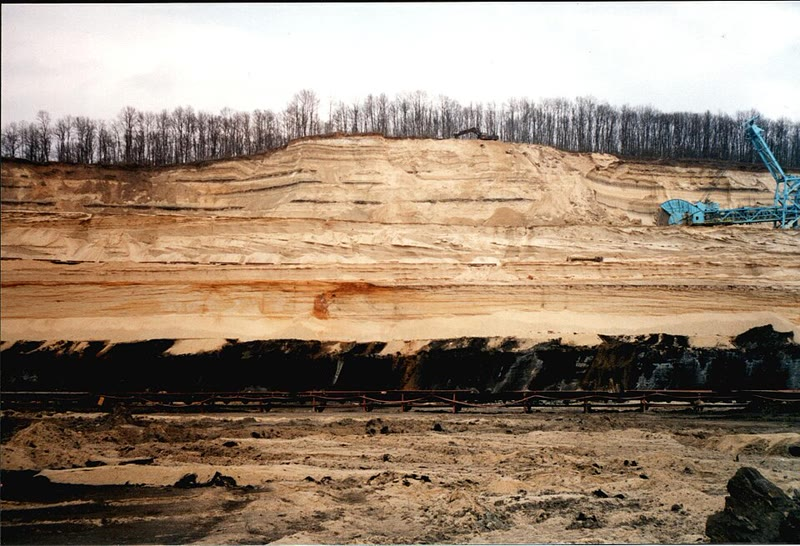
\includegraphics[height=4.0cm]{images/book2/g11-usgs-lignite-bed.jpg}};
\end{tikzpicture}

\medskip
\makebox[0.32\linewidth]{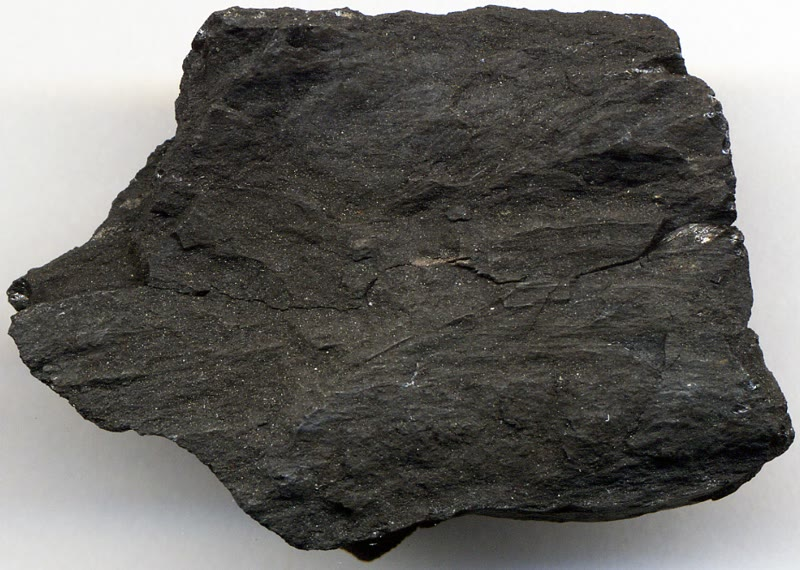
\includegraphics[height=3.2cm]{images/book2/g11-stjohn-lignite.jpg}}\hfill
\makebox[0.32\linewidth]{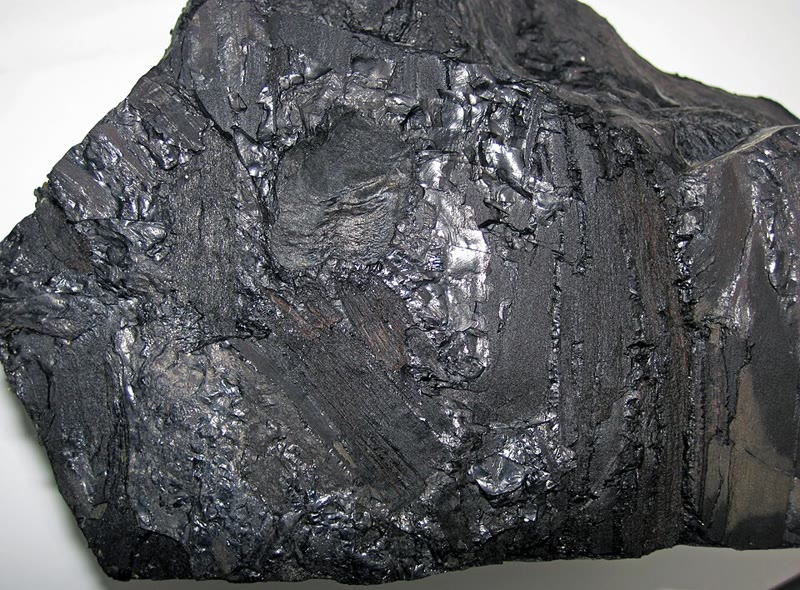
\includegraphics[height=3.2cm]{images/book2/g11-stjohn-bituminous.jpg}}\hfill
\makebox[0.32\linewidth]{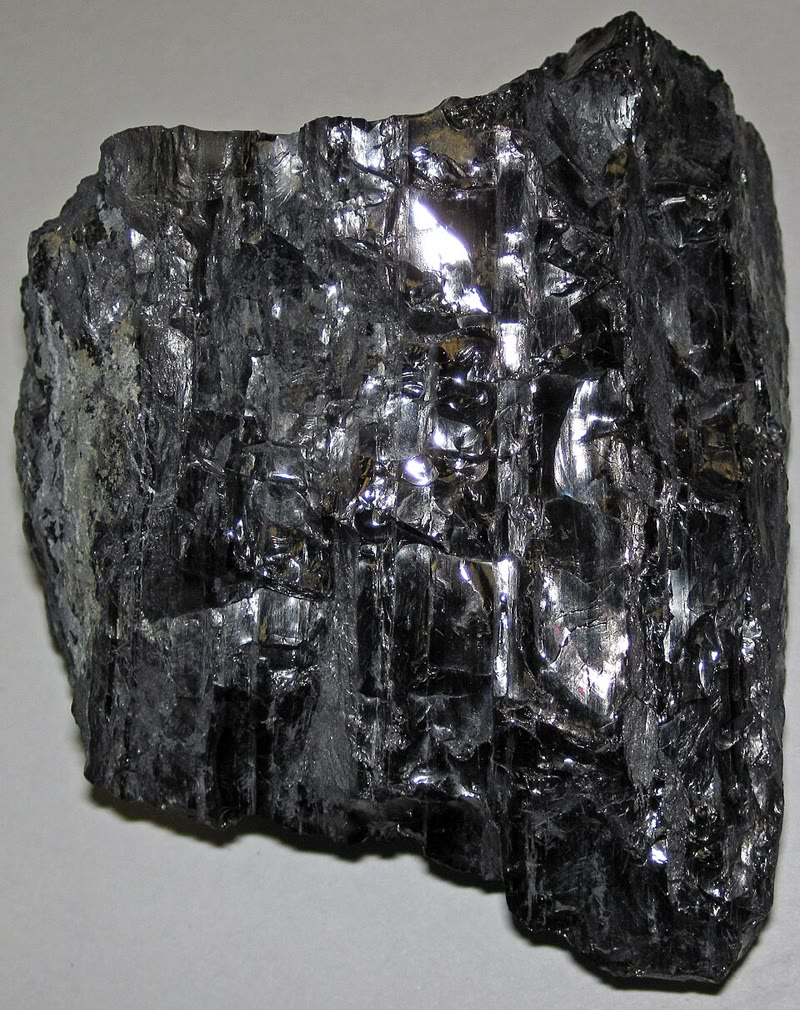
\includegraphics[height=3.2cm]{images/book2/g11-stjohn-anthracite.jpg}}

{\small Em cima, à esquerda: teor de carbono dos \omterm{def:g11:fossil-fuel-geology:coal}{graus de carbonificação} do
\omterm{def:g11:fossil-fuel-geology:coal}{carvão}. Dados: U.S. Energy Information Administration. Em cima, à direita:
uma camada de linhito, a faixa preta sob areias claras, exposta numa mina na
Romênia; fotografia U.S. Geological Survey (domínio público). Embaixo, a
partir da esquerda: linhito, com cerca de \qty{4.5}{cm} de largura,
preto-acastanhado e fosco; \omterm{def:g11:fossil-fuel-geology:coal}{carvão} betuminoso, com fragmentos de plantas
achatados; antracito, preto e vítreo. Fotografias James St.~John
(CC~BY~2.0).}
\end{omfigure}
% ledger: eia:coal-carbon, photo:g11-lignite-bed, photo:g11-coal-ranks

A turfa perde a maior parte do seu volume no caminho. Numa camada de \omterm{def:g11:fossil-fuel-geology:coal}{carvão}
do centro do Utah, a comparação entre a turfa cortada por um antigo canal de
rio e o \omterm{def:g11:fossil-fuel-geology:coal}{carvão} que falta ao lado dá uma razão de espessuras de cerca de
$11{:}1$: cada metro desse \omterm{def:g11:fossil-fuel-geology:coal}{carvão} betuminoso foi um dia uns onze metros de
turfa.
% ledger: ryer80:peat-coal

\section{Exercícios}

\begin{exercise}[$\star$]\label{exo:g11:fossil-fuel-geology:1}
Ponha em ordem as etapas que levam do plâncton ao petróleo numa \omterm{def:g11:fossil-fuel-geology:trap}{armadilha}: a
\omterm{def:g11:fossil-fuel-geology:migration}{migração}; a \omterm{def:g11:fossil-fuel-geology:oil-window}{maturação} na \omterm{def:g11:fossil-fuel-geology:oil-window}{janela do petróleo}; o soterramento sob sedimentos
mais jovens; o plâncton morto se deposita num fundo de mar pobre em
oxigênio; o petróleo se acumula sob uma \omterm{def:g11:fossil-fuel-geology:reservoir}{rocha selante}; a matéria orgânica
vira \omterm{def:g11:fossil-fuel-geology:source-rock}{querogênio} numa lama.
\end{exercise}

\begin{exercise}[$\star$]\label{exo:g11:fossil-fuel-geology:2}
Para cada rocha, diga se ela é mais provavelmente uma \omterm{def:g11:fossil-fuel-geology:source-rock}{rocha geradora}, uma
\omterm{def:g11:fossil-fuel-geology:reservoir}{rocha reservatório} ou uma \omterm{def:g11:fossil-fuel-geology:reservoir}{rocha selante}: (1) um folhelho escuro rico em
matéria orgânica; (2) um arenito bem selecionado com poros ligados; (3) uma
camada de sal; (4) um lamito sem matéria orgânica; (5) um calcário cheio de
cavidades abertas.
\end{exercise}

\begin{exercise}[$\star$]\label{exo:g11:fossil-fuel-geology:3}
Numa bacia, a superfície está a \qty{10}{\degreeCelsius} e o \omterm{def:g11:lithosphere-asthenosphere:geotherm}{gradiente
geotérmico} é de \qty{25}{\degreeCelsius/km}. Entre que profundidades fica a
\omterm{def:g11:fossil-fuel-geology:oil-window}{janela do petróleo}? Qual é a sua espessura?
\end{exercise}

\begin{exercise}[$\star$]\label{exo:g11:fossil-fuel-geology:4}
(1) Ponha o linhito, o antracito, o \omterm{def:g11:fossil-fuel-geology:coal}{carvão} betuminoso e a turfa em ordem
crescente de \omterm{def:g11:fossil-fuel-geology:coal}{grau de carbonificação}. (2) Qual tem o maior teor de carbono?
(3) Qual se formou à maior profundidade e temperatura?
\end{exercise}

\begin{exercise}[$\star$]\label{exo:g11:fossil-fuel-geology:5}
(1) Numa \omterm{def:g11:fossil-fuel-geology:trap}{armadilha}, por que o gás fica acima do petróleo, e o petróleo
acima da água? (2) Por que a rocha acima de um reservatório precisa ser
impermeável? Cite duas rochas que são boas \omterm{def:g11:fossil-fuel-geology:reservoir}{rochas selantes}.
\end{exercise}

\begin{exercise}[$\star\star$]\label{exo:g11:fossil-fuel-geology:6}
Duas bacias têm a mesma temperatura de superfície, \qty{15}{\degreeCelsius}.
A bacia A tem um gradiente de \qty{20}{\degreeCelsius/km}, a bacia B de
\qty{40}{\degreeCelsius/km}. (1) Calcule as profundidades do topo e da base
da \omterm{def:g11:fossil-fuel-geology:oil-window}{janela do petróleo} em cada uma. (2) Uma \omterm{def:g11:fossil-fuel-geology:source-rock}{rocha geradora} fica a
\qty{2}{km} de profundidade nas duas bacias. O que ela produz em cada uma?
(3) Em que bacia um poço precisa ir mais fundo para encontrar petróleo
formado no local?
\end{exercise}

\begin{exercise}[$\star\star$]\label{exo:g11:fossil-fuel-geology:7}
Tome a razão de $11{:}1$ medida no centro do Utah entre a espessura de uma
turfa e a do \omterm{def:g11:fossil-fuel-geology:coal}{carvão} em que ela se transformou. (1) Que espessura de turfa
formou uma camada de \omterm{def:g11:fossil-fuel-geology:coal}{carvão} de \qty{3}{m} de espessura? (2) Suponha que a
turfa se acumulou a \qty{1}{mm} por ano. Quanto tempo ela levou para se
acumular? (3) Por que o pântano precisou estar afundando durante todo esse
tempo?
\end{exercise}

\begin{exercise}[$\star\star$]\label{exo:g11:fossil-fuel-geology:8}
Use o diagrama de história de soterramento da Bacia de Merrow (superfície a
\qty{20}{\degreeCelsius}, gradiente de \qty{30}{\degreeCelsius/km}). A \omterm{def:g11:fossil-fuel-geology:source-rock}{rocha
geradora} estava a \qty{1.2}{km} de profundidade há 120 milhões de anos, a
\qty{2.3}{km} há 95 milhões de anos e a \qty{4.0}{km} há 20 milhões de
anos. (1) Calcule a sua temperatura em cada data. (2) Em cada data, ela
estava imatura, na \omterm{def:g11:fossil-fuel-geology:oil-window}{janela do petróleo} ou na \omterm{def:g11:fossil-fuel-geology:oil-window}{janela do gás}?
\end{exercise}

\begin{exercise}[$\star\star$]\label{exo:g11:fossil-fuel-geology:9}
O topo de um arenito reservatório forma um arco cuja crista fica a
\qty{2400}{m} de profundidade; a sua curva de nível fechada mais profunda
fica a \qty{2580}{m}. Um poço na crista encontra gás até \qty{2450}{m}, e
depois petróleo. (1) Qual é a altura máxima da coluna que a \omterm{def:g11:fossil-fuel-geology:trap}{armadilha} pode
conter? (2) Se a \omterm{def:g11:fossil-fuel-geology:trap}{armadilha} está cheia, qual é a espessura do petróleo?
(3) O petróleo e o gás que continuam chegando depois que a \omterm{def:g11:fossil-fuel-geology:trap}{armadilha} está
cheia: para onde vão?
\end{exercise}

\begin{exercise}[$\star\star$]\label{exo:g11:fossil-fuel-geology:10}
Quando não há nenhuma medição do \omterm{def:g11:fossil-fuel-geology:source-rock}{querogênio}, os geólogos do petróleo têm
considerado madura uma \omterm{def:g11:fossil-fuel-geology:source-rock}{rocha geradora} enterrada sob mais de \qty{3}{km} de
rochas. Com uma superfície a \qty{20}{\degreeCelsius}: (1) Que gradiente põe
\qty{3}{km} no topo da \omterm{def:g11:fossil-fuel-geology:oil-window}{janela do petróleo}? E na sua base? (2) Com os
gradientes de 25 a \qty{34}{\degreeCelsius/km} medidos nos furos de
sondagem, onde fica \qty{3}{km}? A regra é razoável?
\end{exercise}

\begin{exercise}[$\star\star$]\label{exo:g11:fossil-fuel-geology:11}
Três amostras de \omterm{def:g11:fossil-fuel-geology:coal}{carvão} contêm \qty{30}{\percent}, \qty{70}{\percent} e
\qty{92}{\percent} de carbono. (1) Dê o \omterm{def:g11:fossil-fuel-geology:coal}{grau de carbonificação} de cada uma.
(2) Usando as profundidades e as temperaturas dadas no curso, qual foi
enterrada mais fundo? (3) O linhito tem um aspecto fosco e
preto-acastanhado; qual é o aspecto do antracito?
\end{exercise}

\begin{exercise}[$\star\star\star$]\label{exo:g11:fossil-fuel-geology:12}
Entre 120 e 95 milhões de anos atrás, \qty{1100}{m} de lama se acumularam
na Bacia de Merrow. (1) Calcule a taxa de soterramento em metros por milhão
de anos. (2) Com um gradiente de \qty{30}{\degreeCelsius/km}, quantos graus
a \omterm{def:g11:fossil-fuel-geology:source-rock}{rocha geradora} se aqueceu por milhão de anos? (3) Se essa taxa tivesse
continuado, quanto tempo a \omterm{def:g11:fossil-fuel-geology:source-rock}{rocha geradora} teria levado para atravessar toda
a \omterm{def:g11:fossil-fuel-geology:oil-window}{janela do petróleo}? (4) O modelo dá cerca de 66 milhões de anos. Por que
mais?
\end{exercise}

\begin{exercise}[$\star\star\star$]\label{exo:g11:fossil-fuel-geology:13}
Na Bacia de Merrow, a \omterm{def:g11:fossil-fuel-geology:source-rock}{rocha geradora} esteve na \omterm{def:g11:fossil-fuel-geology:oil-window}{janela do petróleo} de cerca
de 117 a cerca de 51 milhões de anos atrás, e o anticlinal que retém o
petróleo se formou há 80 milhões de anos. (1) Suponha que a \omterm{def:g11:fossil-fuel-geology:source-rock}{rocha geradora}
produziu petróleo a uma taxa constante enquanto esteve na janela. Que fração
do seu petróleo se formou depois que a \omterm{def:g11:fossil-fuel-geology:trap}{armadilha} existia? (2) O que
aconteceu com o resto? (3) Se o anticlinal tivesse se formado há 40 milhões
de anos, o que ele poderia conter?
\end{exercise}

\begin{exercise}[$\star\star\star$]\label{exo:g11:fossil-fuel-geology:14}
Tome a história de soterramento da Bacia de Merrow (\cref{exo:g11:fossil-fuel-geology:8}:
\qty{0.4}{km} há 150 milhões de anos, \qty{1.2}{km} há 120, \qty{2.3}{km}
há 95, \qty{3.0}{km} há 66, com a profundidade crescendo de forma
constante entre essas datas), mas numa bacia mais quente: gradiente de
\qty{40}{\degreeCelsius/km}, superfície a \qty{20}{\degreeCelsius}.
(1) Calcule as profundidades do topo e da base da \omterm{def:g11:fossil-fuel-geology:oil-window}{janela do petróleo}.
(2) Calcule as idades em que a \omterm{def:g11:fossil-fuel-geology:source-rock}{rocha geradora} entrou na janela e saiu dela.
(3) O anticlinal ainda se forma há 80 milhões de anos. Ele conteria
petróleo? Gás?
\end{exercise}

\begin{exercise}[$\star\star\star$]\label{exo:g11:fossil-fuel-geology:15}
Uma camada de antracito do Carbonífero aflora hoje na superfície. O
Carbonífero terminou há cerca de 299 milhões de anos. (1) Usando as
profundidades dadas no curso, a que profundidade, no mínimo, a camada foi
enterrada? (2) Com uma superfície a \qty{15}{\degreeCelsius} e um gradiente
de \qty{30}{\degreeCelsius/km}, que temperatura ela atingiu a essa
profundidade? Isso é coerente com a temperatura dada para o antracito?
(3) O que aconteceu com as rochas que ficavam acima dela? Dê um limite
inferior da taxa média, em milímetros por ano, supondo que tudo aconteceu
depois do Carbonífero.
\end{exercise}

\section{Problema: quando a rocha geradora produziu petróleo?}

\begin{problem}[{Problema de fim de semana --- datar o petróleo de uma bacia inventada}]
\label{pb:g11:fossil-fuel-geology:1}
% values (oil_window.py): enter_oil_Ma 116.97, leave_oil_Ma 51.238, T_max 140, T_today 125,
% after_trap_frac 0.43757; ledger ics:base.Jurassic, ics:base.Cretaceous, earle:*, magoon00:tps
Um poço perfurado através da crista de um anticlinal na Bacia de Merrow, uma
bacia inventada, atravessa as camadas de baixo. Datadas pelos seus fósseis,
elas registram como a bacia se encheu. Da mais antiga:
\begin{center}
\small
\begin{tabular}{|l|l|l|}
\hline
\textbf{intervalo (há milhões de anos)} & \textbf{espessura} & \textbf{rochas} \\
\hline
165 a 150 & \qty{400}{m} & folhelho negro rico em matéria orgânica; lamito \\
150 a 120 & \qty{800}{m} & arenito poroso \\
120 a 95 & \qty{1100}{m} & lamito \\
95 a 66 & \qty{700}{m} & giz \\
66 a 35 & \qty{700}{m} & areias e argilas \\
35 a 20 & \qty{300}{m} & areias \\
20 até hoje & \qty{-500}{m} & soerguimento: os \qty{500}{m} de cima erodidos \\
\hline
\end{tabular}
\end{center}
A superfície está a \qty{20}{\degreeCelsius} e o \omterm{def:g11:lithosphere-asthenosphere:geotherm}{gradiente geotérmico} é de
\qty{30}{\degreeCelsius/km}, ambos tomados como constantes. As camadas
conservam a sua espessura depois de depositadas (a compactação é ignorada).
O anticlinal se formou há 80 milhões de anos. Acompanhe o folhelho negro da
base, depositado há 165 milhões de anos.

\medskip
\noindent\textbf{Parte I --- As rochas.}
\begin{enumerate}
  \item Que camada é a \omterm{def:g11:fossil-fuel-geology:source-rock}{rocha geradora}, qual é o reservatório, qual é a \omterm{def:g11:fossil-fuel-geology:reservoir}{rocha
        selante}?
  \item O que tornou o folhelho negro rico em matéria orgânica?
  \item O Jurássico durou de cerca de \num{201.4} a \num{143.1} milhões de
        anos atrás. Em que período a \omterm{def:g11:fossil-fuel-geology:source-rock}{rocha geradora} foi depositada? E o
        arenito?
  \item O que é o \omterm{def:g11:fossil-fuel-geology:source-rock}{querogênio}? Por que o folhelho negro não produz petróleo
        na superfície?
  \item Que espessura de rochas fica por cima da \omterm{def:g11:fossil-fuel-geology:source-rock}{rocha geradora} hoje?
\end{enumerate}

\medskip
\noindent\textbf{Parte II --- O soterramento em função do tempo.}
\begin{enumerate}[resume]
  \item Calcule a profundidade da \omterm{def:g11:fossil-fuel-geology:source-rock}{rocha geradora} há 150, 120, 95, 66, 35 e
        20 milhões de anos, e hoje.
  \item Calcule a taxa de soterramento, em metros por milhão de anos,
        durante cada um dos seis primeiros intervalos.
  \item Quando a \omterm{def:g11:fossil-fuel-geology:source-rock}{rocha geradora} esteve mais funda, e a que profundidade?
  \item Por que a sua profundidade diminuiu nos últimos 20 milhões de anos?
  \item A que profundidade fica hoje a base do arenito?
\end{enumerate}

\medskip
\noindent\textbf{Parte III --- A temperatura em função do tempo.}
\begin{enumerate}[resume]
  \item Calcule a temperatura da \omterm{def:g11:fossil-fuel-geology:source-rock}{rocha geradora} em cada data da
        questão~6.
  \item Entre que profundidades fica a \omterm{def:g11:fossil-fuel-geology:oil-window}{janela do petróleo} nesta bacia?
  \item Entre quais duas datas da questão~6 a \omterm{def:g11:fossil-fuel-geology:source-rock}{rocha geradora} passou de
        \qty{60}{\degreeCelsius}?
  \item Supondo que a sua profundidade cresceu de forma constante nesse
        intervalo, calcule a idade em que ela atingiu \qty{60}{\degreeCelsius}.
  \item Do mesmo modo, calcule quando ela atingiu \qty{120}{\degreeCelsius}.
\end{enumerate}

\medskip
\noindent\textbf{Parte IV --- Na janela, e a armadilha.}
\begin{enumerate}[resume]
  \item Qual é a temperatura mais alta que ela atingiu? O que ela produz
        hoje?
  \item O que aconteceu com o petróleo formado antes que o anticlinal
        existisse?
  \item Supondo que o petróleo se formou a uma taxa constante enquanto a
        \omterm{def:g11:fossil-fuel-geology:source-rock}{rocha geradora} esteve na janela, que fração dele se formou depois
        que o anticlinal existia?
  \item Que fluidos o poço deveria encontrar na crista do anticlinal, e em
        que ordem, de cima para baixo?
  \item Conclua: quando a \omterm{def:g11:fossil-fuel-geology:source-rock}{rocha geradora} entrou na \omterm{def:g11:fossil-fuel-geology:oil-window}{janela do petróleo}?
\end{enumerate}
\end{problem}
